\documentclass{report}
\usepackage{graphicx} % Required for inserting images
\usepackage{todonotes}
\usepackage{amsmath}
\usepackage{amsfonts}
\title{BP - RRR}

\newcommand{\itodo}[1]{\todo[inline]{#1}}
\newcommand{\vtodo}[1]{\todo[inline,color=purple!50!white]{#1}}

\date{January 2025}

\begin{document}

\maketitle

\begin{abstract}
\itodo{Add abstract}
\end{abstract}

\tableofcontents

\section{Introduction}
\label{sec:introduction}

\itodo{write introduction}
Why solving the problem:
- Deep learning models may show "Clever Hans"-like behavior - making use of confounding factors within datasets.
- As demonstrated in~\cite{schramowski2020making}


Following \cite{schramowski2020making}, ...


\section{Theory}
\label{sec:theory}
\itodo{Edit the report. Remove non-proffesional vocabulary}

\subsection{Supervised classification}
\label{subsec:sup-class}
\subsubsection{Neural Network}
Model in Machine Learning refers to the mathematical representation of a process, that has been trained on data.
One of the most important properties of the model is that one way or another it encapsulates the patterns of the data.
Neural network (aka NN) is a specific type of the model in Machine Learning,
which aims to mimic the work patterns of animal brain neurons.
Neural network is built from layers, basic structure of NN is: 1 input layer, 1 output layer,
and multiple hidden layers between the previous two.
Layer is built from nodes, which have relationships with nodes from neighbouring layers.
Each node receives so-called \emph{signals} from connected nodes, processes them and pushes new signal to other connected nodes.
This \emph{signal} is a number, that is the result of \emph{activation function}
applied on \emph{weighted signals from the previous layer}.
Signals are weighted by weights, that are assigned to the corresponding relationship the signal comes from.
When the model is learning or is being trained, what actually happens is that weights on every relationship are adjusted.
\begin{itemize}
 \item Data, that is sent to input layer, is commonly referred to as ``inputs'', ``Xs''.
 \item Data, that are the result of the output layer, is commonly referred to as ``outputs'', ``predictions''.
 \item Data, that are the expected results of processed inputs, is commonly referred to as ``targets'', ``labels'', ``ys''.
\end{itemize}

\vtodo{Introduce also more formally as a parmateric function $y=f_{\theta}(X)$, where $\theta$ are learnable parameters. }
\itodo{Something like ``Relationship between inputs and predictions abstractly speaking is $\hat{y}=f_{\theta}(X)$, where $\theta$ is a vector of learnable parameters.''}

Supervised Learning is a technique, which utilises \emph{labels} to create a model that can predict correct outputs.
Other techniques usually don't rely on \emph{labels}.

To evaluate if the model performs well or bad \emph{loss/cost functions} are defined.
Usually these functions evaluate how much model's predictions are far from ``ground truth'' predictions.
In other words, should we minimize the \emph{loss} produced by the cost function, we may achieve a great performance
of the model.


In order to minimize the loss we use yet another Machine Learning technique called ``Optimizers''.
The most basic optimizing technique is \emph{Stochastic Gradient Descent} aka SGD\@.
During the execution of the SGD the weights are updated as follows (according to~\cite{Li_2018}):
\begin{equation}
 \label{eq:sgd}
 \boldsymbol{\theta}^{[new]} = \boldsymbol{\theta}^{[old]} - \mu \boldsymbol{P} \boldsymbol{\hat{g}}(\boldsymbol{\theta}^{[old]}) \text{,}
 \end{equation}
where $\boldsymbol{\theta}$ is learnable parameters, $\mu$ is learning step/rate, $\boldsymbol{\hat{g}}(\boldsymbol{\theta}^{[old]})$ is gradients of learnable parameters and $\boldsymbol{P}$ is a matrix called ``preconditioner''.
In most of the training sessions $\boldsymbol{P}$ is set to $\boldsymbol{I}$ aka \emph{identity matrix}
- in such case optimizer is called ``plain'' SGD\@.

In our paper we use \emph{Adaptive Moment Estimation} optimizer commonly known as \emph{ADAM}.
This technique is actually a special case of preconditioned SGD, and it is defined as follows (according to~\cite{kingma2017adammethodstochasticoptimization}):
\begin{align}
 m_t = \beta_1 m_{t - 1} + (1 - \beta_1) g_t \\
 v_t = \beta_2 v_{t - 1} + (1 - \beta_2) g_t^2 \\
 \hat{m_t} = \frac{m_t}{1 - \beta_1^t} \\
 \hat{v_t} = \frac{v_t}{1 - \beta_2^t} \\
 \theta_t = \theta_{t - 1} - \mu \frac{\hat{m_t}}{(\sqrt {\hat{v_t}} + \epsilon)} \text{,}
\end{align}
where $t$ is a discrete timestep, $g_t = \nabla_\theta f_t (\theta_{t - 1})$, $\beta_1$ and $\beta_2$ are hyperparameters.
Additionally, it is important to note, that $\beta_i^t$ is $\beta_i$ to the power of $t$, $g_t^2$ indicates the elementwise square $g_t * g_t$.

As the \emph{optimizers} need to calculate gradients for every weight in the model
most of the deep learning frameworks suggest usage of \emph{Automatic Differentiation} (aka AD) tool~\cite{TODO}.
\itodo{I guees we need to describe learning: forward and back propagation??}
\vtodo{Not really. Just say, that the gradients are computed using automatic differentiation and use proper references.}
\itodo{Should I reference to the Pytorch implementation's paper of Automatic Differentiation (https://openreview.net/forum?id=BJJsrmfCZ) or this paper, which describes what it is(https://www.jmlr.org/papers/v18/17-468.html)}

\subsubsection{Cross-entropy loss function}
\label{subsubsec:cross-entropy-loss}
Cross-entropy loss function, a specialised loss function for supervised classification task given by:
\[L = -\frac{1}{N} \sum_{i=1}^{N} \sum_{j=1}^{C} y_{ij} \log(\hat{y}_{ij})
\text{,}\]
where N is number of examples and C is number of classes.

\emph{Cross-entropy loss} function is derived from \emph{Cross entropy} given by (\ref{eq:cross-entropy}),
which quantifies the difference between 2 probability distributions.
It is closely related to data likelihood under \emph{Bernoulli distribution} in such way,
that \emph{Cross entropy} is derived by taking negative logarithm of (\ref{eq:bernoulli-likelihood}).

\begin{equation}
 \label{eq:bernoulli-likelihood}
 P(y | \hat{y}) = \hat{y}^y (1 - \hat{y})^{1-y}
\end{equation}
\begin{equation}
 \label{eq:cross-entropy}
 H(p, q) = -\sum_{x \in \mathcal{X}} p(x) \log q(x)
\end{equation}

\itodo{Im not sure if I should somehow describe it more, maybe suggest an intuition to the reader}
\vtodo{Some details would be nice. E.g. correspondence to Bernoulli likelihoood.}
\itodo{Review resolving of this TODO}

\subsubsection{Convolutional Neural Network}
Convolutional Neural Network (aka CNN) is a type of Neural Network, that is well-suited for image recognition.
It is usually made up of such multiple layers as:
\begin{itemize}
 \item \textbf{Convolutional layers}: layers, which apply convolutional operations to input, using \emph{filters} (aka kernels).
 These kind of operations help to detect complex features such as edges, textures and other patterns.
 \item \textbf{Pooling layers}: layers, which reduce spatial dimensions of the input.
 These operations decrease computational complexity - speed up processing.
 \item \textbf{Activation Function layers}: non-linear activation functions,
 which add non-linearity to the model and help model to learn more complex relationships in the data.
 The most common such layer is \emph{Rectified Linear Unit} (ReLU)
 \item \textbf{Fully connected layers (aka Dense layers)}: this layer connect every neuron to every neuron of the next layer.
\end{itemize}

\subsection{Explanations}
\label{subsec:explanations}

\subsubsection{Grad-CAM}
\label{subsubsec:gradcam}
\emph{Gradient-weighted Class Activation Mapping (Grad-CAM)} is an explanation technique proposed by
\cite[Grad-CAM: Visual Explanations from Deep Networks via Gradient-based Localization]{Selvaraju_2019} paper.
It produces `visual explanation' for decisions of the vast majority of CNN-based models.
It uses the gradients of the target concept flowing into the final convolutional layer resulting into localization map
highlighting regions of the image, which contributed to the prediction of the model.

According to \cite{Selvaraju_2019} the \emph{class-discriminative localization map Grad-CAM $L_{Grad-CAM}^c \in \mathbb{R}^{uxv}$}
for any class $c$ is computed as follows:
\begin{samepage}
    \[\alpha_k^c = \overbrace{\frac{1}{Z} \sum_i^u \sum_j^v}^{\text{global average pooling}}
    \underbrace{\frac{\partial y^c}{\partial A_{ij}^k}}_{\text{gradients via backprop}}\]

    \[L_{Grad-CAM}^c = ReLU(\underbrace{\sum_k \alpha_k^c A^k}_{\text{linear combination}}) \quad \text{,}\]
\end{samepage}
where $y^c$ stands for the score for class $c$, $A^k$ is the $k$-th feature map activations of the convolutional layer, $Z = u * v$.
\itodo{Not really sure if we should the following example: So for example we've got a convolutional layer, which outputs 32 channels of 14 by 14 feature maps, k should be in range [1,32]. Because it was not obvious to me, that feature map activations was referring to every channel individually instead of the tensor of all channels.}

\subsubsection{Guided Grad-CAM}
\label{subsubsec:guided-gradcam}

\emph{Guided Grad-CAM}~\cite{Selvaraju_2019} is an advanced version of \emph{Grad-CAM} (Subsection~\ref{subsubsec:gradcam}),
which focuses on highlighting fine-grained details against \emph{Grad-CAM}'s showing ``relevant'' regions.

Before we dive in how \emph{Guided Grad-CAM} is computed, we should talk about one of the constructs of this method and that is \emph{Guided Backpropagation},
a pixel-space gradient visualization technique proposed by \emph{Springenberg}\cite{springenberg2014striving}.

We take forward pass of the input until the convolutional layer we are interested in as shown on the Figure~\ref{fig:guided_backprop_forward}.
And after that we ``reconstruct'' the image as shown on the Figure~\ref{fig:guided_backprop_backward} and aggregated in equation~\ref{eq:guided-backprop}.

\begin{equation}
 R_i^l = (f_i^l > 0) \cdot (R_i^{l+1} > 0) \cdot R_i^{l+1} \text{,}
 \label{eq:guided-backprop}
\end{equation}
where $R_i^{l+1} = \frac{\partial \text{out}}{\partial f_i^{l+1}}$.
\begin{figure}
 \centering
 \includegraphics[width=0.75\textwidth]{imgs/guided_backpropagation_1}
 \caption{Forward pass of the image}
 \label{fig:guided_backprop_forward}
\end{figure}

\begin{figure}
 \centering
 \includegraphics[width=0.75\textwidth]{imgs/guided_backpropagation_2}
 \caption{Backward pass of the output to ``reconstruct'' the image}
 \label{fig:guided_backprop_backward}
\end{figure}

\emph{Guided Grad-CAM} is a combination of the strength of both techniques.
It is computed as element-wise multiplication of the \emph{Guided Backpropagation}'s ``reconstructed image''
and \emph{Grad-CAM}'s attention map (upsampled to the input image resolution using \emph{bilinear interpolation} according to~\cite{Selvaraju_2019}).

\itodo{Maybe we should cut out Guided Backpropagation into its own subsubsection}

\subsection{Right for the right reasons}
\label{subsec:rrr-theory}
\emph{Right for the right reasons}, the core of our paper, is a loss function for a differentiable model suggested by~\cite{ross2017right} and modified by~\cite{schramowski2020making}.
\itodo{Not sure about this statement as it is valid for now and could be changed as there is CounterExamples method (and maybe others). I would rather say that the core of our paper is research of XIL.}
``Right for the right reasons'' loss (further referred as \emph{RRR loss}) is defined as follows:
\begin{samepage}
 \begin{equation}
  \label{eq:rrr-right-answers}
  L(\theta, X, y, A) = \sum_{n=1}^{N} \sum_{k=1}^{K} -c_k y_{nk} \log (\hat{y}_{nk}) \quad \text{(Right answers)}
  \end{equation}

 \begin{equation}
  \label{eq:rrr-right-reasons}
  + \lambda_1 \sum_{n=1}^{N} \sum_{d=1}^{D} \left( A_{nd} \frac{\delta}{\delta h_{nd}} \sum_{k=1}^{K} c_k \log (\hat{y}_{nk}) \right)^2 \quad \text{(Right reasons)}
 \end{equation}

 \begin{equation}
  \label{eq:rrr-l2-reg}
  + \lambda_2 \sum_{i} \theta_i^2 \quad \text{(Weight regularization)}
  \end{equation}
\end{samepage}
where $\theta$ is a vector of weights, $X$ is the inputs, $y$ is labels, $A$ is binary masks, $c$ is a class weight,
$\hat{y}$ is the predictions and $h$ is feature map of the convolutional layer, usually the last.
$N$ stands for the number of examples, $K$ is for the number of classes our model outputs, $D$ is the number of features in feature map.
RRR loss's right answers in equation's part (\ref{eq:rrr-right-answers}) is the
\emph{Cross-entropy loss} function (Subsection~\ref{subsubsec:cross-entropy-loss}) modified with class weights.
RRR loss's weight regularization in equation's part (\ref{eq:rrr-l2-reg}) is common L2 regularization preventing overfitting of the model.
The novel part is in equation's part (\ref{eq:rrr-right-reasons}), which tries to penalize the gradients of
the convolutional layer from being too large in the regions marked by binary masks.
The $\lambda$ values are used to weight the different regularizations.
According to~\cite{ross2017right} the regularization parameter $\lambda_{1}$ should be set such that the
``right answers'' and ``right reasons'' terms have similar orders of magnitude.

We suggest a modification to this loss function, particularly to the ``right reasons'' equation's part (\ref{eq:rrr-right-reasons}),
and that is an additional sum through the all convolutional layers of the interest as shown in (\ref{eq:rrr-modified}):
\begin{align}
 L(\theta, X, y, A) = \sum_{n=1}^{N} \sum_{k=1}^{K} -c_k y_{nk} \log (\hat{y}_{nk}) \\
 + \lambda_1 \frac{1}{L}\sum_{l=1}^{L} \sum_{n=1}^{N} \sum_{d=1}^{D} \left( A_{nd} \frac{\delta}{\delta h_{nd}^{l}} \sum_{k=1}^{K} c_k \log (\hat{y}_{nk}) \right)^2 \label{eq:rrr-modified} \\
 + \lambda_2 \sum_{i} \theta_i^2
\end{align}
\itodo{maybe add l2 regularization theory subsection}

It is also important to note, that in implementations of RRR loss binary masks are created with the size of the original input,
rather than the size of feature maps of the convolutional layers of interest.
\itodo{statement is really ambitious, as I've got only 2 sources, my implementation and implementation of \cite{ross2017right}}
And during the computation of loss every binary mask is downscaled to the size of each convolutional layer using bilinear interpolation.

\section{Experiments}
\label{sec:experiments}
Before approaching a bigger experiment, we've decided to come up with a simple one, which would show some core
aspects of the introduced methodology and also show us what tools and methods we need to focus our attention to.

So what we want in summary is:
\begin{enumerate}
\item Take a particular dataset for the classification task;
\item Train a model with so-called \emph{common approach};
\item Try out some of the explainers and choose the one, which would offer explanations satisfying our needs;
\item Find a scenario, where model trained with common approach doesn't perform well;
\item Retrain the model using novel approach aka RRRLoss (Subsection~\ref{subsec:rrr-theory});
\item Show that newly trained model rejects confounding factors as part of the classification's explanation.
\end{enumerate}

\subsection{MNIST}
\label{subsec:08-mnist}

Before we dive in the MNIST experiment we should describe our training parameters,
which is applied to most trainings mentioned in this subsection (should training be different, changes would be mentioned):
\begin{itemize}
 \item \textbf{Model architecture}: our model is a sequence of such layers
 (which are shown on Figure~\ref{fig:08_cnn_architecture}: \begin{enumerate}
                                                            \item Convolutional layer with kernel size 3x3, stride=1, padding=1
                                                            \item ReLU layer
                                                            \item MaxPool layer with kernel size 2x2, stride=2
                                                            \item Convolutional layer with kernel size 3x3, stride=1, padding=1
                                                            \item ReLU layer
                                                            \item MaxPool layer with kernel size 2x2, stride=2
                                                            \item Flattening layer from 32x7x7 to 1568
                                                            \item Fully Connected layer from 1568 to 128
                                                            \item ReLU layer
                                                            \item Fully Connected layer from 128 to 2
                                                            \item Softmax layer
 \end{enumerate}
 \item \textbf{Optimizer}: ADAM($\beta_1=0.9; \beta_2=0.999$; learning rate=0.001)
 \item \textbf{Loss function}: Cross Entropy Loss or RRR Loss.
 \item \textbf{Other Training details}: batch size=64, number of epochs=2, train data size=11773,
 test data size=1954
\end{itemize}

\begin{figure}
 \centering
 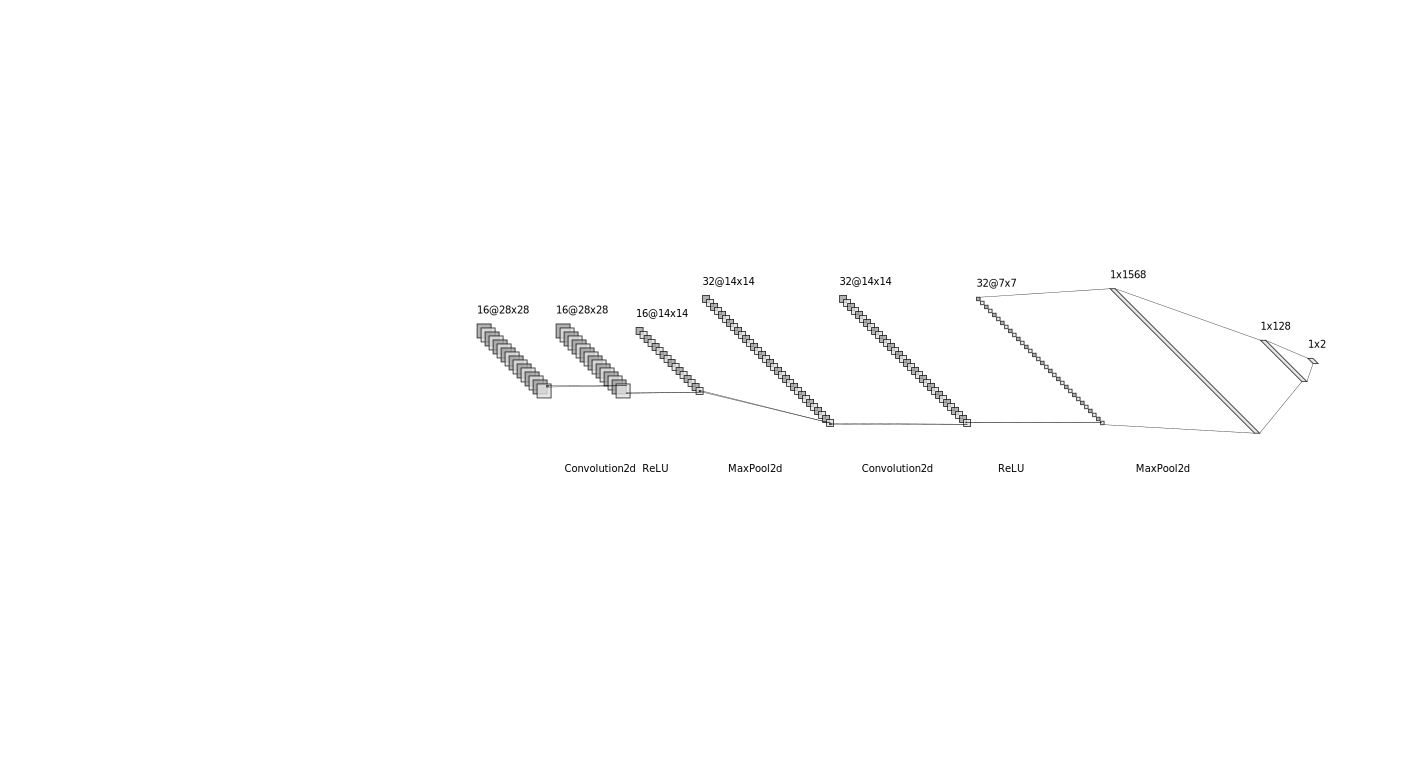
\includegraphics[width=\textwidth]{imgs/08_mnist_cnn}
 \caption{Architecture of the CNN used in MNIST experiment.}
 \label{fig:08_cnn_architecture}
\end{figure}

Thus, we take a standard \emph{MNIST} dataset~\cite{deng2012mnist}
and narrow it down in such way, that it would contain only zeros and eights.
The reason for such a choice is that an intuitive explanation of the difference between such instances should be around
middle part of the image, where eights have ``cross'' as demonstrated on the figure~\ref{fig:08_diff}.
And this is exactly what we expect the explainer to annotate for us as the \emph{right reason} for the classification.

\begin{figure}
 \centering
 \includegraphics{imgs/zero_eight_diff}
 \caption{Intuitive difference between 0 and 8.}
 \label{fig:08_diff}
\end{figure}

\subsubsection{Comparison of explainers}

In this section we're describing our choice of explainer.
The core requirement was to choose the so-called `model-agnostic` explainer,
so we started from Grad-CAM series of explainers and chose basic Grad-CAM (Section~\ref{subsubsec:gradcam}).

The model performs well, and we can clearly see that attention map generated by Grad-CAM (Figure~\ref{fig:gradcam_exp})
has good explanation of what regions of the instances made contributions to prediction, but we cannot exactly tell by
such attention maps what is the difference between given instances, so it is not informative enough.

\begin{figure}
 \centering
 \includegraphics[width=0.5\textwidth]{imgs/exp_2_5_gradcam}
 \caption{Grad-CAM attention map.}
 \label{fig:gradcam_exp}
\end{figure}

That's why we've decided to use Guided Grad-CAM (Section~\ref{subsubsec:guided-gradcam}), which provides more detailed
explanation, than Grad-CAM. As could be seen on Figure~\ref{fig:guided_gradcam_exp}
we've somewhat achieved our goal and that is our model differs zeros and eights by the intuition we proposed earlier on Figure~\ref{fig:08_diff}.

\begin{figure}
 \centering
 \includegraphics[width=0.5\textwidth]{imgs/exp_2_5_guided_gradcam}
 \caption{Guided Grad-CAM attention map.}
 \label{fig:guided_gradcam_exp}
\end{figure}

\subsubsection{Undertrained model's explanations}
We also wanted to see what explanations the model has, if it was undertrained.
That's why instead of the whole training dataset we gave the model 200 samples with 3 epochs.
The accuracy of the model reached $93\%$, after applying Grad-CAM (Subsection~\ref{subsubsec:gradcam})
we were surprised to see (Figure~\ref{fig:gradcam_on_poor_model}),
that the model trained to differ eights from zeros by the background, rather than silhouette of the object.
We presume, that such model will perform worse, should the background filled with noise in real world deployment.
\begin{figure}
 \centering
 \includegraphics[width=0.75\textwidth]{imgs/gradcam_on_poor_adam}
 \caption{Grad-CAM applied on the undertrained model}
 \label{fig:gradcam_on_poor_model}
\end{figure}

\subsubsection{Artificial dataset}
In previous subsection we showed that our trained model was trained well and its explanations of the classification tasks seem
to be good too, but what actually happens when we gather such dataset, that may have additional \emph{not necessarily helpful} patterns? \itodo{Maybe we should find some sources to support our argument here?}

We decided to add a dot to every sample of eight in our dataset, as shown on Figure~\ref{fig:dotted_ds} to represent
a dataset gathered from within \emph{limited environment}.

\begin{figure}
 \centering
 \includegraphics[width=0.5\textwidth]{imgs/zero_eight_dot}
 \caption{A pair of zero and "dotted" eight.}
 \label{fig:dotted_ds}
\end{figure}

We have trained the model on such dataset, applied Guided Grad-CAM and, although the accuracy reaches same values as the
model trained on unmodified dataset, the explanation of classifying eights mostly comes from the given dot
(Figure~\ref{fig:guided-gradcam-dotted}).
Furthermore, when evaluating the model on unmodified dataset, accuracy may fall down to $60\%$ as described in Table~\ref{tab:avg-accuracy-rrr}.
\begin{table}
 \label{tab:avg-accuracy-rrr}
 \centering
 \caption{Table showing average accuracy of the model trained with RRR loss function throughout 3 executions.}
\begin{tabular}{|l||c|c|}
 \hline
 Average accuracy with RRR loss & Train dataset & Test dataset \\
 \hline \hline
 $\lambda_1=0;\lambda_2=0$ & $100\%$ & $65,8\%$ \\
 \hline
 $\lambda_1=2;\lambda_2=0$ & $99,8\%$ & $97,9\%$ \\
 \hline
\end{tabular}
\end{table}

\begin{figure}
 \centering
 \includegraphics[width=0.5\textwidth]{imgs/exp_4_dotted_8_gradcam}
 \caption{Guided Grad-CAM on dotted dataset.}
 \label{fig:guided-gradcam-dotted}
\end{figure}

\subsubsection{RRR}
At this point of our experiment we retrain our model with the \emph{same} hyperparameters, \emph{same} model architecture
and \emph{same} optimizer, but we use ``right for the right reasons'' loss function (Section~\ref{subsec:rrr-theory})
instead of previously used Cross-entropy loss.
As for the needed binary masks by RRR method, we define them as follows: 1) put 1s in the region of the dot; 2) 0 otherwise.

\begin{figure}
 \centering
 \includegraphics[width=0.5\textwidth]{imgs/exp_4_dotted_guided_gradcam_rrr}
 \caption{Guided Grad-CAM on dotted dataset. Model trained with RRR.}
 \label{fig:guided-gradcam-dotted-rrr}
\end{figure}

As could be seen on the Figure~\ref{fig:guided-gradcam-dotted-rrr} our model learnt to reject the dot, furthermore it
learnt to differ zeros and eight by the intuition we suggested in Figure~\ref{fig:08_diff}

\section{Plans and improvements}
\label{sec:plans-improvements}
\itodo{Slight issue in codebase: cam overlay does not work for guided Grad-CAM}
\itodo{try out learning, when binary masks are really costly to make, in other words, model learns and sometimes queries
binary mask}
\itodo{Counterfactual explanations suggested by Grad-CAM paper sounds interesting. I think we might use it, but not sure for what.}
\itodo{This seems interesting: \cite[At the other extreme, when A is a matrix of all 1s, it encourages the model to have small gradients with respect to its inputs; this can improve generalization on its own Drucker and Le Cun, 1992.]{ross2017right}}

\vtodo{I would be interested in a sensitivity study: i.e. what if there is $n$ samples of 8s that no not have the dot? How many $n$ I need to get to the accuracy (and right reason) comparable to RRR? }

\section{Conclusion}
\label{sec:conclusion}

what works, what not, how to proceed...


\bibliographystyle{plain}
\bibliography{bib}
\end{document}
